\documentclass[11pt]{article}
\usepackage{graphicx}
\usepackage{listings}
\usepackage[utf8]{inputenc}
%Gummi|065|=)
\title{\textbf{Tarea}}
\author{Juan Carlos Olivier Jasso}
\date{}
\begin{document}

\maketitle

\section{ANN-what}
Las redes neuronales artificales area de inteligencia computacional, inspirado en la paradigma computacional. Inspirados en neuronas biologicas, para la resolucion de problemas asociados reconocimiento , clasificación, aproximación , la predicción y la optimización. Presentan habilidades para el aprendizaje automatico, generalizacion y abstraccion.\\
Algunas Caracteristicas 	

\begin{itemize}
\item Aprendizaje: Reaccion a su entorno
\item Generalizacion: cambios en las variables del entorno
\item Abstraccion: buscar las caracteristicas principales de la informacion
\end{itemize}

\emph{Componentes basicos}

\begin{itemize}
\item elementos de proceso , llamadas neuronas
\item Activation reglas para cada neurona.
\item Interaction reglas entre las neuronas (topografía o topología) normas 
\item La información sobre el entorno en el que está incrustada la ANN (ejemplos)
\end{itemize}

\emph{Entrenamiento}\\ 
Aprender del medio a traves de ejemplos representativos, el entrenamiento consiste en ajustar los pesos por un conjunto de entradas y salidas que se desean, un auto- organización se produce cuando las salidas deseadas son desconocidos.
Normalmente , los valores de entrada y de salida son numéricos . Pueden ser entero, flotante o de tipo binario .

\newpage

\section{ANN-concepts}

\textbf{Clasificacion: }

\begin{itemize}
\item redes neuronales de una sola capa
\item redes neuronales multi-capa
\item redes neuronales recurrentes
\item Combinacion de las previas
\end{itemize}


\emph{Redes neuronales de una sola capa}

\begin{itemize}
\item Organizadas en una sola linea
\item Obtienen informacion directamente del mundo exterior
\item Salida es directamente a las ANN
\end{itemize}

\emph{Redes MLP}

\begin{itemize}
\item Organizacion no linear
\item La salida es la ultima linea y son calculados desde la primer neurona
\end{itemize}

\emph{Algoritmo "Back Propagtion"}

Es un entrenamiento supervisado
El objetivo es encontrar los valores de los pesos que se
minimizar el error cuadrático medio obtenido de la
la producción real y deseada de la MLP . Esto es un
algoritmo basado en gradiente

\emph{Mapas de auto-organizacion}

El propósito de auto- organización es descubrir patrones o características significativas en los datos de entrada , sin la ayuda de un maestro.Cada uno de N neuronas de entrada se conecta a todas las neuronas de salida M de un modo de alimentación hacia adelante
Hay conexiones laterales inhibidoras implícitas entre las neuronas en la capa de salida
Cada neurona en la capa ouput tiene algunos efectos en sus Vecinos neuronas .
\newpage

\section{ANN-solutions}

En la actualidad, hay un sinnúmero de modelos y arquitecturas de ANN. El diseño de una ANN implica tomar ventajas de las características del dominio del problema y las capacidades de ANN para resolver el problema.
\\
\\

Hay varias salidas en un MLP , uno para cada clase, por lo tanto, un proceso para decidir la respuesta que se requiere.La mejor manera de elegir una clase, es el cálculo de la distancia euclidiana de la salida de la red a cada clase posible. La muestra pertenece a la clase con la distancia más lento.

\textbf{Proceso:}
\begin{enumerate}
\item Diseñar cuidadosamente el vector característico , la elección de las medidas apropiadas y procesamiento previo de ellos, si es necesario.
\item Analizar la conveniencia de normalizar las características , si la varianza en sus magnitudes son altos
\item Recoger la mayor cantidad de datos posible . Es mejor tener un número similar de ejemplos para cada clase posible
\item Dividir los datos en 2 o 3 juegos : conjunto de entrenamiento , validación establecidos y conjunto de pruebas
\item El número de nodos de entrada es igual al tamaño del vector de característica,El número de nodos de salida es igual al número de clases en en la solución,	Decidir un número inicial de nodos ocultos en el PLM 
\item Comenzar a entrenar a su red . Si disminución error total lentamente o no disminuyen , tratar con los nodos más o menos ocultos
\end{enumerate}
.\\\\
Recurrentemente las redes neuronales:
\begin{itemize}
\item Son sistemas dinámicos que aprenden de los datos 
\item Si bien entrenados , que son capaces de oscilar en una manera estable 
\item Los algoritmos de entrenamiento de RNN son dificil de implementar y controlar 
\item Son muy potentes.
\end{itemize}
\newpage

\section{ANN-examples}

\emph{Proceso principal:}
\begin{enumerate}
\item Obtener los datos para ser utilizados
\item Define la red
\item Entrena la red
\item Utiliza y evalua el rendimiento de la red
\end{enumerate}

\begin{figure}[htp]
\centering
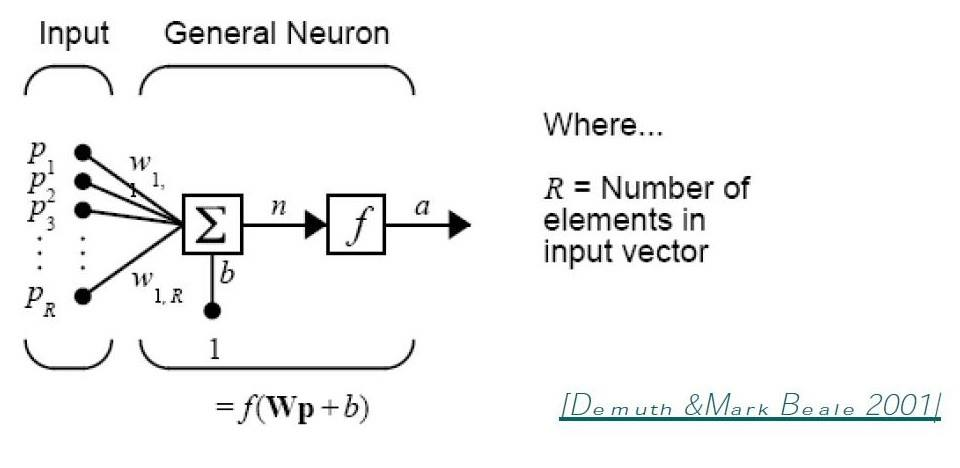
\includegraphics[width=9.5cm]{2.jpg}
\label{fig:lion}
\end{figure}


Despues de estos pasos se podra utilizar completamente la red

Representación NN caja de herramientas de un MLP

\begin{figure}[htp]
\centering
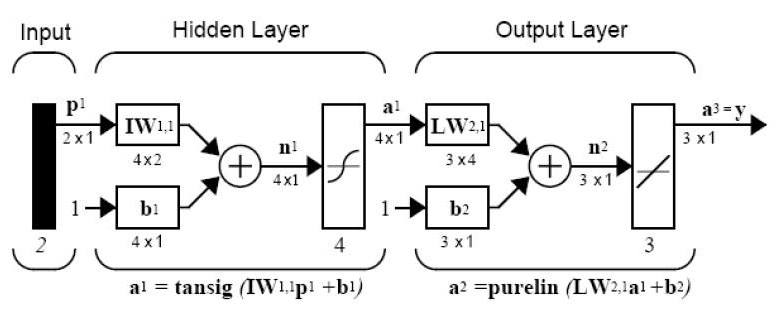
\includegraphics[width=9.5cm]{1.jpg}
\label{fig:lion}
\end{figure}

\newpage

\section{hopfield}
\lstinputlisting{hopfield.cpp}

\newpage

\section{threshold}
\lstinputlisting{threshold.cpp}

\end{document}
